\documentclass[12pt,a4paper]{article}
\usepackage{task}

\newcommand{\contestName}{MateInfoUB}
\newcommand{\contestDates}{18 Mai 2025}
\newcommand{\contestPlace}{Facultatea de Matematic\v a-Informatic\v a}
\newcommand{\contestRound}{Runda Final\v a}
%\newcommand{\contestRound}{Rund\v a de Test}
\newcommand{\statementLanguage}{Rom\^ an\v a (Oficial)}
\newcommand{\taskShortName}{Iele}


\definecolor{Brown}{cmyk}{0,0.81,1,0.60}
\definecolor{OliveGreen}{cmyk}{0.64,0,0.95,0.40}
\definecolor{CadetBlue}{cmyk}{0.62,0.57,0.23,0}
\definecolor{lightlightgray}{gray}{0.9}

\lstset{
% language=C++,                             % Code langugage
basicstyle=\ttfamily,                   % Code font, Examples: \footnotesize, \ttfamily
keywordstyle=\bfseries,        % Keywords font ('*' = uppercase)
commentstyle=\color{gray},              % Comments font
columns=flexible,
% numbers=left,                           % Line nums position
% numberstyle=\tiny,                      % Line-numbers fonts
% stepnumber=1,                           % Step between two line-numbers
% numbersep=5pt,                          % How far are line-numbers from code
% backgroundcolor=\color{lightlightgray}, % Choose background color
% frame=none,                             % A frame around the code
% tabsize=2,                              % Default tab size
% captionpos=b,                           % Caption-position = bottom
% breaklines=true,                        % Automatic line breaking?
% breakatwhitespace=false,                % Automatic breaks only at whitespace?
% showspaces=false,                       % Dont make spaces visible
% showtabs=true,                         % Dont make tabls visible
}


\setlength{\parskip}{0pt}

\begin{document}
% Tex fragment for task statement headers
% Usage:
%       % Defining parameters required for header
%       \newcommand{\contestName}{Name of the Contest Series}
%       \newcommand{\contestDates}{Month 1 -- 8 20XX}
%       \newcommand{\contestPlace}{City, Country}
%       \newcommand{\contestRound}{Day 1}
%       \newcommand{\statementLanguage}{en (US)}
%       \newcommand{\taskShortName}{task_short_name}
%       % Tex fragment for task statement headers
% Usage:
%       % Defining parameters required for header
%       \newcommand{\contestName}{Name of the Contest Series}
%       \newcommand{\contestDates}{Month 1 -- 8 20XX}
%       \newcommand{\contestPlace}{City, Country}
%       \newcommand{\contestRound}{Day 1}
%       \newcommand{\statementLanguage}{en (US)}
%       \newcommand{\taskShortName}{task_short_name}
%       % Tex fragment for task statement headers
% Usage:
%       % Defining parameters required for header
%       \newcommand{\contestName}{Name of the Contest Series}
%       \newcommand{\contestDates}{Month 1 -- 8 20XX}
%       \newcommand{\contestPlace}{City, Country}
%       \newcommand{\contestRound}{Day 1}
%       \newcommand{\statementLanguage}{en (US)}
%       \newcommand{\taskShortName}{task_short_name}
%       \input{header.tex}
%


%--------------------- tools ----------------------
\makeatletter
% \expandafter for the case that the parameter is given in a command
\newcommand{\escapeUnderscores}[1]{\expandafter\@repl@underscores#1_\relax}
\def\@repl@underscores#1_#2\relax{%
    \ifx \relax #2\relax
        % #2 is empty => finish
        #1%
    \else
        % #2 is not empty => underscore was contained, needs to be replaced
        #1%
        \textunderscore
        % continue replacing
        % #2 ends with an extra underscore so I don't need to add another one
        \@repl@underscores#2\relax
    \fi
}
\makeatother
% -------------------------------------------------

\vspace*{-3em}\hspace*{-.5cm}
\begin{tabular}{ccl}
    \hspace{1mm}
\includegraphics[width=2.2cm,valign=b]{logo.jpeg}
    & 
    \begin{minipage}[b]{10cm}
        \setlength{\baselineskip}{1.05\baselineskip}
        \sffamily
        \makebox[0pt][l]{\bfseries \large \contestName}  \\
        \contestDates \\ 
        \contestPlace
    \end{minipage}
    & 
    \begin{minipage}[b]{3.7cm}
        \begin{flushright}
            \makebox[0pt][r]{\ttfamily \bfseries \large \escapeUnderscores{\taskShortName}}  \\[.2em]
            \sffamily
            \contestRound \\
            \statementLanguage
        \end{flushright}
    \end{minipage}
\end{tabular} 
\hrule height .06em
%


%--------------------- tools ----------------------
\makeatletter
% \expandafter for the case that the parameter is given in a command
\newcommand{\escapeUnderscores}[1]{\expandafter\@repl@underscores#1_\relax}
\def\@repl@underscores#1_#2\relax{%
    \ifx \relax #2\relax
        % #2 is empty => finish
        #1%
    \else
        % #2 is not empty => underscore was contained, needs to be replaced
        #1%
        \textunderscore
        % continue replacing
        % #2 ends with an extra underscore so I don't need to add another one
        \@repl@underscores#2\relax
    \fi
}
\makeatother
% -------------------------------------------------

\vspace*{-3em}\hspace*{-.5cm}
\begin{tabular}{ccl}
    \hspace{1mm}
\includegraphics[width=2.2cm,valign=b]{logo.jpeg}
    & 
    \begin{minipage}[b]{10cm}
        \setlength{\baselineskip}{1.05\baselineskip}
        \sffamily
        \makebox[0pt][l]{\bfseries \large \contestName}  \\
        \contestDates \\ 
        \contestPlace
    \end{minipage}
    & 
    \begin{minipage}[b]{3.7cm}
        \begin{flushright}
            \makebox[0pt][r]{\ttfamily \bfseries \large \escapeUnderscores{\taskShortName}}  \\[.2em]
            \sffamily
            \contestRound \\
            \statementLanguage
        \end{flushright}
    \end{minipage}
\end{tabular} 
\hrule height .06em
%


%--------------------- tools ----------------------
\makeatletter
% \expandafter for the case that the parameter is given in a command
\newcommand{\escapeUnderscores}[1]{\expandafter\@repl@underscores#1_\relax}
\def\@repl@underscores#1_#2\relax{%
    \ifx \relax #2\relax
        % #2 is empty => finish
        #1%
    \else
        % #2 is not empty => underscore was contained, needs to be replaced
        #1%
        \textunderscore
        % continue replacing
        % #2 ends with an extra underscore so I don't need to add another one
        \@repl@underscores#2\relax
    \fi
}
\makeatother
% -------------------------------------------------

\vspace*{-3em}\hspace*{-.5cm}
\begin{tabular}{ccl}
    \hspace{1mm}
\includegraphics[width=2.2cm,valign=b]{logo.jpeg}
    & 
    \begin{minipage}[b]{10cm}
        \setlength{\baselineskip}{1.05\baselineskip}
        \sffamily
        \makebox[0pt][l]{\bfseries \large \contestName}  \\
        \contestDates \\ 
        \contestPlace
    \end{minipage}
    & 
    \begin{minipage}[b]{3.7cm}
        \begin{flushright}
            \makebox[0pt][r]{\ttfamily \bfseries \large \escapeUnderscores{\taskShortName}}  \\[.2em]
            \sffamily
            \contestRound \\
            \statementLanguage
        \end{flushright}
    \end{minipage}
\end{tabular} 
\hrule height .06em

\section*{Creaturi 3: Ielele}


\begin{center}
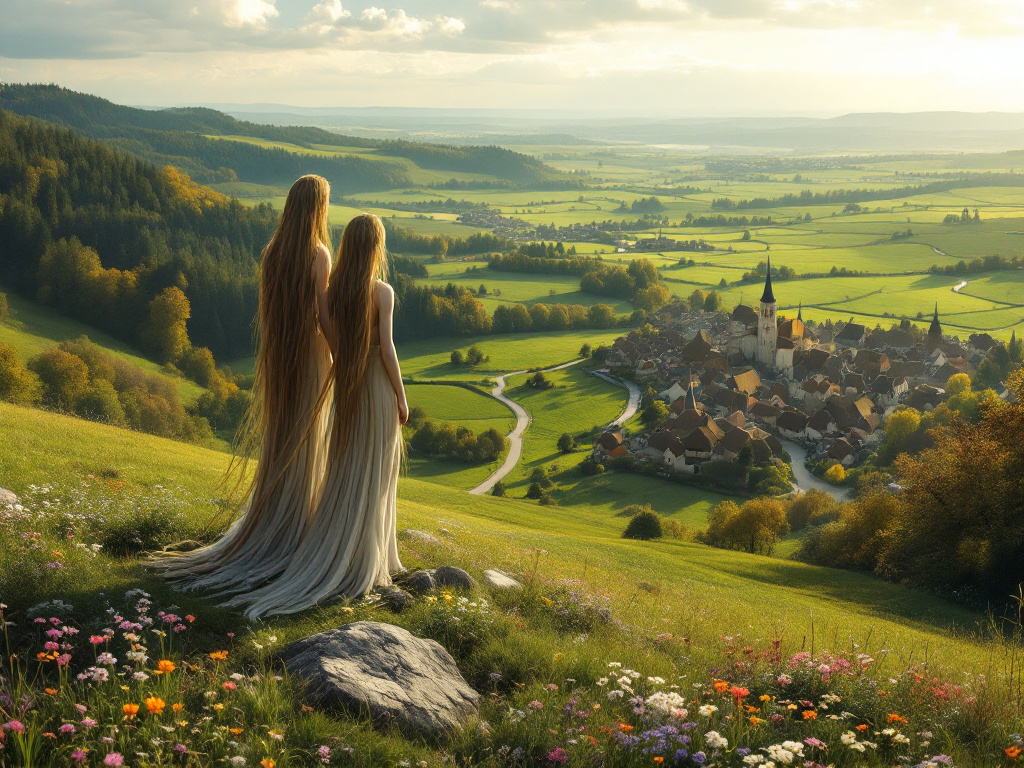
\includegraphics[scale=0.15]{iele.jpg}
\end{center}

Ielele s-au întâlnit în clar de lună pentru horă. Dar vai, pădurea lor fermecată a fost tăiată de săteni, pentru lemne de foc. Furioase, ielele vor să se răzbune. 

\vspace{1em}

În poiana în care ielele trăiesc există $N$ sate, conectate prin $N - 1$ drumuri, în așa fel încât din oricare sat se poate ajunge în oricare alt sat. Fiecare drum are o lungime, exprimată ca un număr natural între $1$ și $M$.

\vspace{1em}

Ielele se întreabă: \textit{Câte parcursuri există între sate, pentru care lungimile drumurilor formează o permutare a numerelor de la $1$ la $M$?}

\vspace{1em}

Un \textit{parcurs} este o cale între două sate care urmează drumurile fără a trece de două ori prin același drum. Cu alte cuvinte, este o succesiune de drumuri care leagă două sate fără a face bucle sau a se întoarce. Un \textit{parcurs} este considerat egal cu parcursul invers.

\vspace{1em}

Ajutați-le să calculeze numărul de parcursuri posibile.

\subsection*{Date de intrare}

Pe prima linie se găsesc numerele $N$ și $M$, cu semnificația din enunț.

Pe următoarele $N - 1$ linii se găsesc câte 3 numere $A$, $B$ ($1 \leq A, B \leq N$) și $L$ ($1 \leq L \leq M$), semnificând că există un drum de lungime $L$ între satul $A$ și satul $B$.

\subsection*{Date de ieșire}

Pe unica linie afișati numărul cerut. 

\subsection*{Constrângeri}

\begin{itemize}
    \item $1 \leq N \leq 10^5$.
    \item $1 \leq M < N$.
    \item Se garantează că datele din input sunt corecte.
\end{itemize}


\subsection*{Subtask-uri}

\begin{enumerate}
    \item ($20$ de puncte) $1 \leq N \leq 1000$.
    \item ($20$ de puncte) $M = 2$.
    \item ($20$ de puncte) $M = 3$.
    \item ($20$ de puncte) Există un parcurs care trece prin toate satele.
    \item ($20$ de puncte) Nicio constrângere suplimentară.
\end{enumerate}

\subsection*{Exemplu}

\begin{tabular}{|@{}p{0.5\textwidth}@{}|@{}p{0.5\textwidth}@{}|}
\hline
\multicolumn{1}{|c|}{\bfseries Input Standard (\textit{cin})} &
\multicolumn{1}{c|}{\bfseries Output Standard (\textit{cout})} \\
\hline
\begin{textQuoteCell}
6 3
1 2 1
2 3 2
3 4 3
3 5 1
2 6 3
\end{textQuoteCell} &
\begin{textQuoteCell}
2
\end{textQuoteCell} \\    
\hline
\end{tabular}
\vspace{1em}

\subsection*{Explicație}

Există două parcursuri valide:
\begin{itemize}
    \item Parcursul \code{6 - 2 - 3 - 5}, și
    \item Parcursul \code{4 - 3 - 2 - 1}.
\end{itemize}

Nu există niciun alt parcus ale cărui lungimi de drumuri să formeze o permutare a numerelor de la $1$ la $3$.

\end{document}